
\chapter{绪论}
\label{chap:introduction}
\section{研究背景与意义}
	互联网自二十世纪九十年代从诞生、发展,到现在已经演化为人类社会的必需品。但是,后互联网时代又是个性化时代\citep{Personalization1},需要一种系统精确刻画每个用户的兴趣爱好并能不动声色的在主页上表现出来,我们把这种提供个性化服务的系统系统统称为推荐系统。推荐系统是一种比搜索引擎更人性化、个性化的系统服务,不需要用户主动提供关键词,因此它能满足用户的更多的潜在需求,尤其当用户自己都无法精准描述自身需求的时候\citep{recmd-system}。第一代推荐系统以亚马逊为代表,作为一个电子商品平台,一方面有数以万计的商品需要被用户了解、熟悉和购买,另一方面有数以亿计的用户无法找到称心如意的商品。推荐系统通过构建用户和商品之间的桥梁,每年为亚马逊贡献近三十个百分点的创收!由此可见推荐系统能帮助用户快速发现有用的商品信息,具体来讲,首先推荐系统通过分析用户的历史行为每个用户进行独一无二的画像建模\citep{demo-data},目的有俩个:1,熟悉每个用户和他们的潜在需求;2,把拥有相同品味的用户归为一类群体,这样一来所有人的需求总和就可能是其中一个人的潜在需求,方便企业卖出更多的商品。随着用户终端设备的普及,出现了诸如淘宝、美团、滴滴、今日头条等互联网平台,几乎包办了人们衣食住行的方方面面,人们因为可选择性太多而出现了“选择性困难”的症状,这其实就是信息过载时代的具体表现形式。也就是说,在这个数据爆炸时代,无论是作为信息消费者的普通用户,还是作为信息生产者的提供商,都面临着日益严峻的挑战,现代人每天面临着从各种不必要的数据中找到有用的商品,其实是在浪费生命。每一个有追求、有理想的现代人,真的需要好好的设计人生,以一种精要的方式摒弃不必要之事,而这也是林语堂先生所说的生之智慧。笔者曾有过这样的一种购物体经历:笔者在淘宝商城购买一台笔记本电脑,花费了一上午的时间才浏览、比较完所有的 thinkpad 品牌商家店面,如\autoref{fig:hl_taobao}。
	\begin{figure}
		\centering
		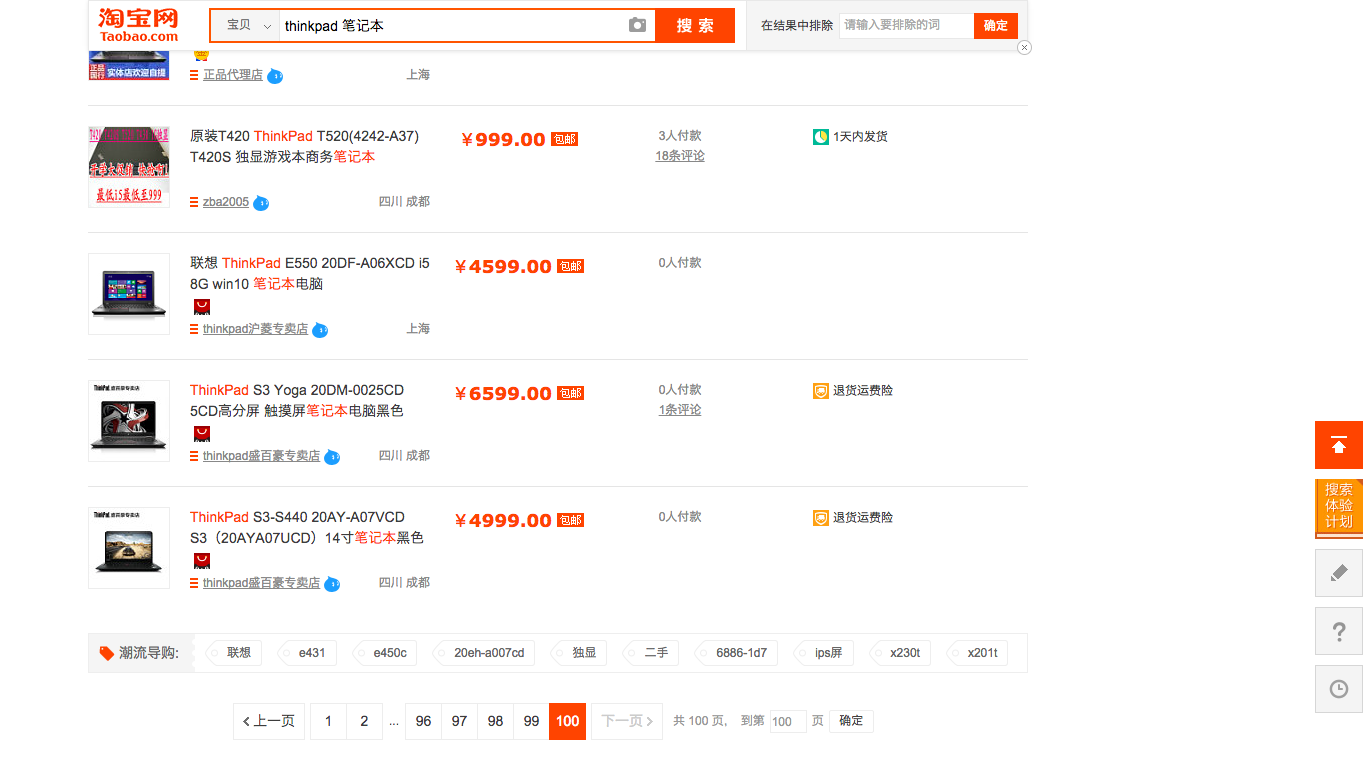
\includegraphics[width=0.9\textwidth]{hl_taobao}
		\figcaption{淘宝购物搜索图}
		\label{fig:hl_taobao}
	\end{figure}
	对于传统的推荐系统,首先,需要积累足够多的商品信息,因为只有尽可能的在基于所有的商品大局观上,才有可能得出比较正确的商品推荐候选集合;其次,需要尽可能积累用户的行为样本数据,因为这些样本将会是推荐统计假设检验的唯一数据标准,统计学之所以常让人意外,就是因为人们只能得到部分样本,而部分样本只是包含了事情的部分信息,于是就有扭曲事情本质的趋势,因此,精度是推荐系统最重要的指标之一,后文会详细介绍如果通过用户画像和用户兴趣提升推荐系统的精度;最后就是甄别,哪些商品对哪些用户有着非同寻常的吸引力,其实对于一个用户来讲,平台上存在的绝大多数商品,包括数据、资源和他人观点,都没有什么价值,只有少数商品效果非凡,影响巨大,推荐系统的核心就是算法\citep{date-mining},通过算法甄别无意义的多数,只留下有意义的少数。总之,通过算法分析用户兴趣,分析商品特性,对用户跟所有商品的关联度打分、排序、取topN,然后给出推荐结果。

	但是,传统的推荐系统也有一些问题,典型的有数据稀疏问题、新用户问题、马太效应、实时推荐问题和用户兴趣变动问题。数据稀疏问题的本质就是商品信息数据过于膨胀,即使是骨灰级用户也没办法穷尽百分之一的商品,因此大多数的用户-商品相关值都是零,这不利于推荐系统做出正确的推荐结果;新用户问题又叫冷启动问题,指一个用户刚刚注册登录,推荐系统没有与此人相关的信息,于是就没有方法做出推荐;马太效应是指越热门的商品越有被推荐的趋势,这种情况其实不是一件好事,因为:1,商品营收不平衡会增加平台的风险性,如果平台大多数营收的贡献来自于极少类明星商品,一旦这类商品发生问题,平台也会有问题;2,根据2/8原则,冷门商品虽然营收少,但它们的基数大,潜力无限;实时推荐问题是指用户从浏览到购买这段时间一般很短,而推荐系统需要打时间差,在用户点击之后、购买之前的这段时间做出推荐,但这是很难实现的,客观原因是工程上需要一定计算时间的;用户兴趣变动问题是指用户兴趣是一个动态的过程,有可能随着季节周期性变动,有可能随着年龄发散性变化,推荐系统需要及时收集数据,保持对用户兴趣的最优拟合。

	基于这些问题的存在,笔者基于推荐系统实现了用户画像模块和用户兴趣探索模块,用以解决传统推荐系统所面临的种种问题,并帮助推荐系统做出更好的推荐结果。用户画像模块其实就是回归了问题的本质:以人为本,用数据说话。通过分析、收集所有与用户有关的数据,为每个用户建立、维护一个独一无二的用户画像,用户画像的最大优点在于它能主动收集用户的基本人口数据、长期兴趣和短期兴趣,而且用户画像中的信息是动态更新的,也就是说随着时间的推移,用户的兴趣在逐渐改变,用户画像里的兴趣标签也会随之改变,最大程度上保证了用户兴趣的连续性和变化性;用户兴趣探索模块包括三个原则:1,用户和潜在感兴趣商品的关联度很低,这保证了探索的商品都是用户从前没有看见过的;2,用户满意度很高,即通过量化用户行为,包括点击次数、滑屏次数、滑屏频率、滑屏时长、点赞、分享等行为,得出用户的满意度;3,潜在商品的标签是小众的、冷门的标签,因为热门商品是没必要也不需要做探索的。

\section{推荐系统的简介}
推荐系统的研究其实是个交叉学科,因为其跟很多早期的基础领域的研究相关,比如认知科学\citep{cognitive-science},信息检索\citep{info-retrieval}和预测理论\citep{Forecast-principle}。随着数据时代的到来,研究人员开始研究如何利用用户对商品的行为数据来预测用户的兴趣,同时为用户提供推荐服务\citep{cf-sn}。近些年来,推荐系统越来越开始成为一个专门的研究课题,到2005年左右为止推荐系统的研究还是集中在基于user、item的协同过滤算法,在工业界目前应用最具有影响力的算法应该就是亚马逊的协同过滤算法\citep{Amazon-cf}。推荐系统推荐有俩个原则:1,给用户的推荐的商品不能与用户购买过的商品重复;2,不能与用户刚浏览过的商品太相关,否则这些商品会让用户有种千篇一律的感觉。

	\subsection{推荐系统的产生与发展}
	随着计算机存储技术以摩尔定律指数增长,信息的传播也开始爆发式的迅猛发展起来,我们这个时代的人类社会进入了一个崭新的大数据信息时代:互联网和物联网几乎无处不在,影响人类的衣食住行等方方面面,因此颠覆性的更改了人们的生活方式,在典型的互联网共享经济平台,一个用户既代表了消费者,也代表了生产者,就如笔者在滴滴出行的角色,平时上下班打车,属于运力消费者,周末开车做网约车司机,则变身为运力生产者。但是不好的一方面也开始浮现,曾几何时笔者发现自己社交账号开始多起来,数量之多以至于没办法记住每个账号的密码。这就是Web 2.0时代的一个副作用---让人们疲于奔命的把生活浪费在刷各种动态、信息,忙于各种无脑点赞、分享,而没有时间思考。社交化网络媒体如微信、微博的异军突起,导致互联网中的信息数据中充满了广告和噪声,而普通用户一般缺少过滤、屏蔽噪声的主观意愿和技术能力,不仅使其信息检索的时间成本巨大,也会让其在茫茫多的数据海洋里迷失自我,这就是信息过载问题的根源所在\citep{info-overload, info-overload:1}。作为非常重要的技术手段,推荐系统和搜索引擎为用户解决信息过载提供了不可或缺的保障。倆者的不同之处在于:搜索引擎是分散的、被动的,用户需要先输入关键词,搜索引擎根据关键字在服务器后台进行信息检索,利用算法获得最优的匹配信息并展示给用户。但我们更多时候遇到的问题是,并不能精确描述自己的需求,而这就是推荐系统的强项,因为推荐系统是主动收集用户平日中一点一滴的数据,以至于用户不需要提供明确的需求,推荐系统只是通过分析用户的历史行为数据就可以“猜出”用户的意图,因此,如果我们把推荐系统和搜索引擎看作为两个互补的技术手段,那么效果一定很棒。

	推荐系统最开始的概念,应该是在1995年由美国人工智能协会\citep{recmd-history}上的Robert Armstrong教授首先提出,不仅如此,Armstrong教授还不遗余力的推广了一个推荐系统的原型系统。受其启发,推荐系统的研究工作开始起步并发展壮大。第一个商用推荐系统应该属于Yahoo网站的个性化入口MyYahoo。到了21新世纪,随着电子商务的风起云涌,推荐系统的研究与应用开始水涨船高,包括eBay、taobao、Amazon、youtube\citep{recmd-youtube}等各大电子商务网站都有了自己的推荐系统。2006年美国的Netflix\citep{recmd-netflix}在网上公开了一个推荐算法竞赛,设立了丰厚的奖金,选手通过利用Netflix公开了的真实网站中的一部分数据,包含用户对电影的评分,利用数据挖掘算法预测哪些用户会购买哪些电影。2014年阿里举办了阿里大数据竞赛,笔者所在团队参加了初赛选拔并顺利进入决赛,阿里公开了其部分用户三个月的浏览、收藏、购买商品数据,选手可以利用阿里天池计算资源做出预测,阿里大数据竞赛有效地推动了学术界和产业界对推荐算法的兴趣,很多有效的算法在此阶段被提了出来。总体说来,一个成功的个性化推荐系统的应用主要表现在以下几个方面:
		\begin{enumerate}[(1)]
		\item 将潜在用户转变为购买者:用户在浏览的同时并不意味着一定是要消费,也许只是看看,遇到合适就买,没有就算。个性化推荐系统的职责之一是能够洞察用户的潜意识,帮助用户找到其感兴趣的商品,从而促成购买过程。
		\item 提高平台的连带销售能力:有时候个性化推荐系统需要一点联想能力,如用户购买了手机,那么推荐手机壳就是一种明智的联想,会让用户产生“你懂我”的感觉。
		\item 提高客户对平台忠诚度:个性化推荐系统就是那个时时刻刻为用户着想的机器人,每一次推荐只是那么一点点,不是很多,但都很好,这种依赖就是俞军先生所说的体验壁垒,对于用户来讲,从滴滴出行换到优步,功能还是原来的功能,只是用户习惯的打车方式都变了,以至于无法接受优步。
		\end{enumerate}

	\subsection{推荐系统的应用}
	对于诸如Linkedin的社交网络,推荐系统改变用户扩展人脉的模式和方法,而这是基于一种假设:你的朋友的朋友有可能就是你的朋友。对于诸如淘宝的电商平台,搜索提供的静态体验,并不足以让用户产生购买欲望,推荐系统加强了交互,包括用户和商品、用户和用户,一个人的消费可能带动一群人模仿,成就了一种极致的营销模式\citep{user-interest}。对于诸如滴滴出行的网约车平台,给定某一时刻、起始经纬度、终点经纬度、车型,根据推荐算法一定会有一个最优派单,使得司机和乘客所得的好处,远远大于平台的抽成费用,形成了我们所说的三方共赢。

	随着网络社交的深入人心,用户不再满足于单纯的获取信息,而是与网络上的其他用户进行关注、聊天和互动。国外著名的社交网络就有Twitter、Facebook等,国内的社交网络有微信、微博等。在社交网站中用户不再是一个静止端点,而是与他人有错综复杂关系的社交网络。对于微信来说,最重要的资源应该就是用户之间的关联。这其中的关系可能是多层次的、多维度的、按时间序列走的,关联的因素可能是是亲人、好友、同学、同事,也可能只是网络中的萍水之交,如都是QQ黄金会员。因此,用户之间的关联应该有一个权重,表明了用户之间的紧密度、信任度,一个用户的好友可能是另一个好友的亲戚,因此推荐系统有助于帮助用户挖掘潜在的熟人。

\section{用户画像的简介}
	用户,指企业的潜在消费者,是构成现有用户的大部分群体的统称。画像,是对一个用户的可视化、客观的描述。用户画像就是能够客观、可视化地描述潜在消费者的模型。用户画像建模的关键工作就是为用户打上合适的标签,标签通常是人为规定,且具有高度精炼的特征标识,如消费能力、偏好、年龄、性别等,将所有用户标签综合起来,抽象出本质,如忠诚度、消费度、满意度等,基本就可以勾勒出该用户的商业消费轮廓。
	\subsection{用户画像的产生背景}
	当互联网步入信息时代后,用户行为数据的极大丰富性给企业及消费者的消费行为带来一系列问题与变革。最大的问题在于电子商务的用户数量相比传统商务,膨胀了成百上千个数量级,单纯依靠人工方式已对其无解,2015上半年,我国网民已达到6.68亿,预计年底能够顺利突破7亿,其中使用手机上网人群占整体88.9\%,而手机上网存在着独特性、唯一性和私密性的特点,每个人的手机都是一套独特的生态系统。最大的变革莫过于,消费者的一切行为信息都是可数字化,随着大数据工程技术的日益精湛,带宽、计算资源、存储资源也变得极大丰富起来。这使得企业有能力把专注点回归到问题的本质,即利用信息化管理方式为每位用户建立一个档案,根据用户的生活习惯、消费行为和社会属性等信息,抽象出的一个标签化的用户模型用以精准刻画用户,基于此进而充分挖掘用户潜在的商业价值,随着用户使用时间越长,模型就越能积累多的数据,也越能精确把握用户的消费习性,反过来越能促使用户的消费行为,形成一个良性循环,至此用户画像的概念也就深入企业和用户之心。

	\subsection{用户画像的应用}
	用户画像的本质就是了解企业的用户,然后完善产品运营提升用户体验,提升盈利,用户画像可以为包括推荐系统、运营推广、策略制定等提供数据支持。除此之外,用户画像可以帮助企业寻找潜在目标用户,在与用户的交互上了解其偏好,促成购买,实现精准运营和营销,用户画像改变了以往闭门造车式的商业交易模式,通过事先调研用户需求反馈,设计制造出更适合用户的产品。具体来讲,用户画像的应用包括:
	\begin{itemize}
	\item 完善及扩充用户信息:用户画像代表了用户的信息全貌,因此寻找足够多的数据是用户画像建模的前提条件。我国在各方面都是很大的长尾市场,互联网很大程度上弥补了信息的不对称,移动互联网能把信息精准送达到任意一个用户面前,尽管如此,根据2/8原则还是导致了大多数的用户和商品的数据是空缺着的。同时,在实际中用户的信息也可能提供得不尽完整,如对于没有填写性别信息的用户,用户画像可以通过用户兴趣探索模块,生成用户数据,可见,用户画像不仅消费数据,也可以生成数据。
	\item 打造健康的生态圈:在掌握用户信息的基础上,电子商务平台就可以对自身的状况进行分析,从相对宏观的角度刻画用户种群的分布,从基础上把握市场的生态环境,挖掘出商品的最大价值,帮助企业提高收入。例如笔者曾经发现,通过与当前热门电影保持同步,通过适时发布作品引导传播、跟进推广周边手机主题,可以很好的带动用户的消费行为,用户的消费与此同时也刺激了第三方设计师紧跟时尚潮流,尽可能第一时间发布引领流行的作品。
	\item 支撑推荐系统的精准推荐:精准推荐的前提是对用户的清晰认知。在实际场景中,影响用户对商品的使用黏度的因素很多,在这种情况下,利用用户画像可以对用户的“贴身跟踪”就能及时发现薄弱环节,因此从用户打开应用网上商店到退出使用,其间的每一步情况都被记录在案:哪一天退出的,哪一步退出的,退出之后“跳转”到什么软件等等。据此,用户画像也实现了用户另外一个纬度的归类,分清哪部分是忠实用户,哪部分可能是潜在的忠实用户,哪些则是已经流失的;更进一步来看流失的原因:因为代金券没有了流失?主题包质量不好流失?这些都是下一步精准推荐的依据,无论是基于兴趣的推荐提升用户价值,精准的广告投放提升商业价值,还是针对特定用户群体的内容运营,用户画像都是其必不可少的基础支撑。
	\item 市场安全领域的应用:有时候商家会通过各种活动形式的补贴来获取用户、培养用户的消费习惯,但同时也催生一些通过刷排行榜、刷红包的用户,这些行为距离欺诈只有一步之遥,但他们的存在严重破环了市场的稳定,侵占了活动的资源。其中一个有效的解决方案就是利用用户画像沉淀方法设置促销活动门槛,即通过记录用户的注册时间、历史登陆次数、常用IP地址等,最大程度上隔离掉僵尸账号,保证市场的稳定发展。
	\end{itemize}

\section{工程背景}
	小米科技有限公司作为国内发展较快的互联网企业,活跃用户过亿,移动端用户比例高,有着大量的用户和丰富的用户行为,这些为推荐系统的应用和优化提供了不可或缺的条件,我们基于MIUI主题应用商店开发的手机主题推荐系统,作为用户和主题包之间的桥梁,体现出超强的变现能力。但现有的手机主题推荐系统也面临着一些问题。
	\begin{enumerate}[(1)]
	\item 新用户冷启动问题:当一个新用户进入一个站点时,我们对他的兴趣爱好还一无所知,这时如何做出推荐是一个很重要的问题。现有的机制是向用户推荐那写普遍反映比较好的物品,也就是说,推荐完全是基于物品的,这就会使热门的商品越来越热,冷门的商品越来越冷,代价就是加剧了热门商品的马太效应。

	\item 数据稀疏问题:通过观察我们发现只有约20\%的用户有过多于5款/日主题的浏览记录,意味着大多数用户的消费处于待挖掘状态。与此同时,我们发现只有约20\%的主题包有过多于10次/日的浏览次数,意味着大多数主题包的消费处于待挖掘状态,又是一个“蛋和鸡”的问题:要形成好的推荐,首先需要有大量的用户行为支持,这样才能得到足够多的推荐数据,这里问题的关键在于推荐系统如何首先能在数据稀疏的情况下给出优质的服务,打破闭环。

	\item 不断变化的用户喜好:这个问题主要分为俩类:1、用户一直喜欢某种类型的主题包,只是长时间没有机会接触,如一位男性用户喜欢美少女主题包款式,虽然不会主动查找,但如果不经意看到一款制作精美的美女主题包,可能还是会购买,这就是用户的长期兴趣。2、用户之前喜欢某种类型的主题包,之后转为喜欢另外一类主题包,如用户刚开始喜欢清纯系,后来转为温柔系,这时如果向用户推荐温柔系主题包更有可能被其接受,这就是用户的短期兴趣。

	\item 重复推荐的问题:手机主题包属于电子虚拟商品,它的特性是第一次下载需要购买,之后下载则免费,现有的推荐系统会重复推荐用户之前购买过的主题,导致占用有限的推荐位来显示无法变现的信息,并且会给用户一种不专业、不智能的体验。

	\item 其他问题:如隐性喜好\citep{latent-cf}、商品长尾性\citep{long-tail},相对来讲这些问题引起的关注度比较小。
	\end{enumerate}

	我们发现,如果在底层数据仓库层和推荐系统之间加一个用户画像模块,会有效提升推荐系统的各项性能。1、对于新用户冷启动问题、数据稀疏问题,关键是收集足够多的用户基本信息,在没有或者只有少量用户行为的情况下依靠用户画像对用户推荐比较合理的主题。2、对于不断变化的用户喜好,我们通过用户画像存储用户中长期兴趣,通过用户兴趣探索获得用户短期兴趣,并针对手机主题市场的特点,利用线性衰减算法融合用户画像和用户兴趣探索,使得推荐结果能兼顾俩者。3、对于重复推荐的问题,我们在用户画像中维护一个白名单,用来存储用户曾购买过的所有主题信息,格式为(userId, itemId, buyTime)这样的三元组,避免向用户推荐已购买过的主题。除此之外,我们也通过探索用户小众兴趣提升推荐系统的长尾发掘能力,加强了对小众主题包的推荐力度。主要思路是分析用户所有的行为数据,针对占大多数的冷门主题(即包含小众标签的主题)会赋予一个倾斜因子,这样会使得冷门主题更有可能被探索出来。

\section{推荐系统开源项目介绍}
工欲善其事,必先利器,关于大数据,有很多令人兴奋的事情,但如何分析、利用好如此多的数据也带来了很多困惑。好在开源观念盛行的今天,有一些在大数据领域领先的免费开源技术可供利用,在这里我们用到的开源工具包括:Redis、Hive、Kafka等流行的大数据存储、计算工具。

\section{论文结构}
	本文的其余正文内容由以下章节组成:
	\begin{itemize}

	\item 第二章是综述了用户画像的推荐系统,对用户画像的研究现状做了介绍,然后介绍了用户画像在推荐系统的应用。
	\item 第三章讨论了手机主题推荐系统的架构设计与技术实现,简单的介绍了用户画像与用户兴趣探索的作用,和其在推荐系统中的作用。
	\item 第四章讨论了用户画像模块,包括用户画像数据类型,用户画像的建模,最后给出了实验与分析。
	\item 第五章介绍了用户兴趣探索模块,包括用户数据的存储和处理,用户兴趣探索模型的俩个关键概念:长尾标签和用户满意度,然后介绍了用户画像和用户兴趣探索的融合的原理;最后给出了实验与分析。
	\end{itemize}